% TODO: 1) Четче проговорить разницу между ранней и поздней материализацией











%%%%%%%%%%%%%%%%%%%%%%%%%%%%%%%%%%%%%%%%%
% Beamer Presentation
% LaTeX Template
% Version 1.0 (10/11/12)
%
% This template has been downloaded from:
% http://www.LaTeXTemplates.com
%
% License:
% CC BY-NC-SA 3.0 (http://creativecommons.org/licenses/by-nc-sa/3.0/)
%
%%%%%%%%%%%%%%%%%%%%%%%%%%%%%%%%%%%%%%%%%

%----------------------------------------------------------------------------------------
%	PACKAGES AND THEMES
%----------------------------------------------------------------------------------------

\documentclass{beamer}

\mode<presentation> {

% The Beamer class comes with a number of default slide themes
% which change the colors and layouts of slides. Below this is a list
% of all the themes, uncomment each in turn to see what they look like.

%\usetheme{default}
%\usetheme{AnnArbor}
%\usetheme{Antibes}
%\usetheme{Bergen}
%\usetheme{Berkeley}
%\usetheme{Berlin}
%\usetheme{Boadilla}
%\usetheme{CambridgeUS}
%\usetheme{Copenhagen}
%\usetheme{Darmstadt}
%\usetheme{Dresden}
%\usetheme{Frankfurt}
%\usetheme{Goettingen}
%\usetheme{Hannover}
%\usetheme{Ilmenau}
%\usetheme{JuanLesPins}
%\usetheme{Luebeck}
\usetheme{Madrid}
%\usetheme{Malmoe}
%\usetheme{Marburg}
%\usetheme{Montpellier}
%\usetheme{PaloAlto}
%\usetheme{Pittsburgh}
%\usetheme{Rochester}
%\usetheme{Singapore}
%\usetheme{Szeged}
%\usetheme{Warsaw}

% As well as themes, the Beamer class has a number of color themes
% for any slide theme. Uncomment each of these in turn to see how it
% changes the colors of your current slide theme.

%\usecolortheme{albatross}
%\usecolortheme{beaver}
%\usecolortheme{beetle}
%\usecolortheme{crane}
%\usecolortheme{dolphin}
%\usecolortheme{dove}
%\usecolortheme{fly}
%\usecolortheme{lily}
%\usecolortheme{orchid}
%\usecolortheme{rose}
%\usecolortheme{seagull}
%\usecolortheme{seahorse}
%\usecolortheme{whale}
%\usecolortheme{wolverine}

%\setbeamertemplate{footline} % To remove the footer line in all slides uncomment this line
%\setbeamertemplate{footline}[page number] % To replace the footer line in all slides with a simple slide count uncomment this line

%\setbeamertemplate{navigation symbols}{} % To remove the navigation symbols from the bottom of all slides uncomment this line
}

\usepackage[utf8]{inputenc}
\usepackage[russian]{babel}
\usepackage{cmap}


\usepackage{verbatim}
\usepackage{fancybox}
\usepackage{ulem}
\usepackage{tikz}
\usetikzlibrary{positioning}
\usepackage{scalefnt}
\usetikzlibrary{arrows,shapes,positioning,shadows,trees,calc,backgrounds,fit,positioning}

\usepackage{graphicx} % Allows including images
\usepackage{booktabs} % Allows the use of \toprule, \midrule and \bottomrule in tables
\usepackage{textcomp}
\usepackage{listings}
\usepackage{color}
\usepackage{xcolor}
\usepackage{changepage}

\definecolor{mygreen}{rgb}{0,0.6,0}
\definecolor{mygray}{rgb}{0.5,0.5,0.5}
\definecolor{mymauve}{rgb}{0.58,0,0.82}

\lstset{ %
  backgroundcolor=\color{white},   % choose the background color; you must add \usepackage{color} or \usepackage{xcolor}
  basicstyle=\footnotesize,        % the size of the fonts that are used for the code
  breakatwhitespace=false,         % sets if automatic breaks should only happen at whitespace
  breaklines=true,                 % sets automatic line breaking
  captionpos=b,                    % sets the caption-position to bottom
  commentstyle=\color{mygreen},    % comment style
  deletekeywords={...},            % if you want to delete keywords from the given language
  escapeinside={\%*}{*)},          % if you want to add LaTeX within your code
  extendedchars=true,              % lets you use non-ASCII characters; for 8-bits encodings only, does not work with UTF-8
  frame=single,                    % adds a frame around the code
  keepspaces=true,                 % keeps spaces in text, useful for keeping indentation of code (possibly needs columns=flexible)
  keywordstyle=\color{blue},       % keyword style
  language=Octave,                 % the language of the code
  morekeywords={*,...},            % if you want to add more keywords to the set
  numbers=left,                    % where to put the line-numbers; possible values are (none, left, right)
  numbersep=5pt,                   % how far the line-numbers are from the code
  numberstyle=\tiny\color{mygray}, % the style that is used for the line-numbers
  rulecolor=\color{black},         % if not set, the frame-color may be changed on line-breaks within not-black text (e.g. comments (green here))
  showspaces=false,                % show spaces everywhere adding particular underscores; it overrides 'showstringspaces'
  showstringspaces=false,          % underline spaces within strings only
  showtabs=true,                  % show tabs within strings adding particular underscores
  stepnumber=1,                    % the step between two line-numbers. If it's 1, each line will be numbered
  stringstyle=\color{mymauve},     % string literal style
  tabsize=4,                       % sets default tabsize to 2 spaces
  %title=\lstname                   % show the filename of files included with \lstinputlisting; also try caption instead of title
}

\graphicspath{{./figures/}}

%----------------------------------------------------------------------------------------
%	TITLE PAGE
%----------------------------------------------------------------------------------------

\title[Обработка и исполнение запросов: лекция 6]{Обработка и исполнение запросов в СУБД (Лекция 6) \\~\\ Колоночные СУБД: введение и диск-ориентированные системы\\~\\ v6} % The short title appears at the bottom of every slide, the full title is only on the title page

\author{Георгий Чернышев} % Your name
\institute[ВШЭ] % Your institution as it will appear on the bottom of every slide, may be shorthand to save space
{
Высшая Школа Экономики \\ % Your institution for the title page
\medskip
\textit{chernishev@gmail.com} % Your email address
}

%\date{\today} % Date, can be changed to a custom date

\date{7 октября 2020 г.}

\begin{document}

\begin{frame}
\titlepage % Print the title page as the first slide
\end{frame}

\begin{comment}
\begin{frame}
\frametitle{Overview} % Table of contents slide, comment this block out to remove it
\tableofcontents % Throughout your presentation, if you choose to use \section{} and \subsection{} commands, these will automatically be printed on this slide as an overview of your presentation
\end{frame}
\end{comment}

\begin{frame}
\frametitle{Колоночная СУБД: идея в первом приближении}

\begin{figure}[htb]
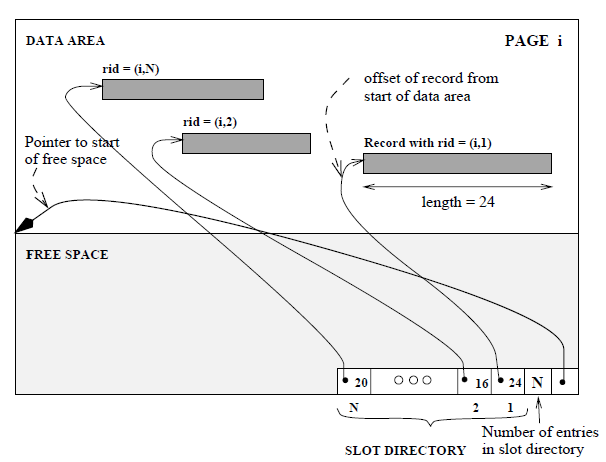
\includegraphics[width=\textwidth,height=0.70\textheight,keepaspectratio]{slotted.png} 
\footnote{\tiny{Изображение взято из \cite{Ramakrishnan2000}}}
 \end{figure}    

\begin{itemize}
  \setlength\itemsep{1em}
  \item Надо считывать с диска меньше данных!
\end{itemize}

\end{frame}


\begin{frame}
\frametitle{Краткая история колоночного подхода}

В основновном по \cite{Harizopoulos2009}:

\begin{itemize}
  \setlength\itemsep{1em}
  \item[<1985] Типы: 
  \begin{itemize}
    \item TOD, Cantor;
    \item индустриальные RAPID, TAXIR;
    \item иногда к ним относят и KDB хотя там не СУБД;
    \item тогда отнесем и элементы компьютеров пятого поколения;
  \end{itemize}
  \item[1985] Две работы Copeland и соавторов: DSM vs. NSM;
  \item[1990] Коммерциализация подхода через Sybase IQ;
  \item[<2000] Hardware-ориентированные работы про поколоночную обработку;
  \item[\textasciitilde 2005] Расцвет исследований, появление стартапов;
  \item[\textasciitilde 2010] Принятие большими игроками, выпуск своих продуктов;
  
\end{itemize}

\end{frame}

\begin{frame}
\frametitle{Предпосылки к популяризации}

Один из важнейших вопросов области баз данных: ``One size fits all?''.\\

\begin{itemize}
  \setlength\itemsep{1em}
  \item Новые запросы, деление на OLAP и OLTP, повышение роли OLAP систем, запрос на них со стороны индустрии \cite{Chernishev2013};
  \item Изменения в оборудовании (разберем на следующей лекции).
\end{itemize}

Актуализация OLAP:

\begin{itemize}
  \setlength\itemsep{1em}
  \item рынок OLAP систем составлял в 2006 году около 6 миллиардов долларов, тогда как в 98 году он составлял всего 2 миллиарда;
  \item По информации TWDI (The Data Warehousing Institute) за прошедшее десятилетие* на порядок выросли и объемы обрабатываемых данных;
  \item Дополнительно можно отметить появление собственно термина OLAP (1993), создание OLAP Council (1995). 
\end{itemize}

 
\end{frame}


\begin{frame}
\frametitle{OLAP и OLTP нагрузки}

{\scriptsize

\begin{table}
\begin{center}
%\begin{tabular}{|c|c|}
\begin{tabular}{|p{0.45\linewidth}|p{0.45\linewidth}|}
\hline
OLAP & OLTP \\
\hline
Запросы заранее неизвестны & Шаблоны запросов известны заранее, например транзакция по оплате услуги или по добавлению пользователя \\
\hline
Запросы могут затрагивать десятки таблиц & Запросы затрагивают малое количество таблиц \\
\hline
Пакетное обновление или полное отсутствие обновления данных & Запросы обновляют данные, при этом делают это на лету \\
\hline
Сложные запросы, требующие оптимизации & Запросы простые~--- не содержат сложных операций, таких как соединение и агрегирование, а значит и не сильно зависят от оптимизации \\
\hline
Большой результат запроса~--- тысячи и миллионы записей & Результат запроса мал~---  десятки или сотни записей \\
\hline
Низкоселективные запросы & 	Высокоселективные запросы~--- результатом будет малая часть исходного отношения \\
\hline
Запрос затрагивает отдельные атрибуты из сотен или даже тысяч атрибутов таблицы & Запрос затрагивает все атрибуты таблицы \\
\hline
Малое количество клиентов~--- десятки или сотни, меньшая важность параллелизма & Запросы поступают параллельно, от большого числа клиентов \\
\hline
\end{tabular}
\end{center}
% \caption{Два типа нагрузок в СУБД}
%\begin{center}\textbf{Два типа нагрузок в СУБД}\end{center}
\end{table}
}

\end{frame}


\begin{frame}
\frametitle{Предшественники колоночных систем}

Работы Copeland et al:

\begin{itemize}
  \item N-ary Storage Model (NSM)~--- стандартный подход;
  \item Decomposition Storage Model (DSM)~--- каждый атрибут в отдельном файле, нужно много соединений.
\end{itemize}

\begin{tikzpicture}[remember picture,overlay]
    \node[xshift=-9cm,yshift=-7.3cm] at (current page.north east)  {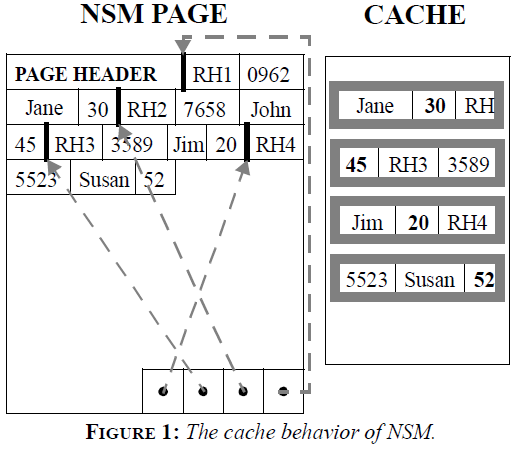
\includegraphics[width=4cm]{nsm.png}};  
    
\end{tikzpicture}

\begin{tikzpicture}[remember picture,overlay]
       \node[xshift=-3cm,yshift=-7.3cm] at (current page.north east) {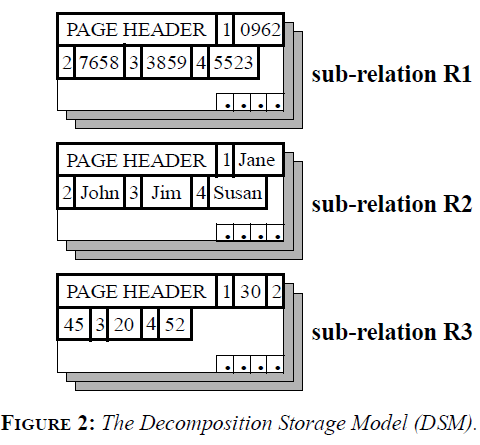
\includegraphics[width=4cm]{dsm.png}};
    
\end{tikzpicture}



\end{frame}


\begin{frame}
\frametitle{Предшественники колоночных систем}

Несколько работ из начала нулевых, buffer pool:

\begin{itemize}
  %\setlength\itemsep{1em}
  \item PAX ~--- статика, в памяти
  \item Data Morphing ~--- динамика, в памяти;
  \item Clotho  ~--- диск, MEMS, динамика;
  \item Fractured Mirrors ~--- диск, две копии NSM и DSM.
\end{itemize}

\begin{tikzpicture}[remember picture,overlay]
    \node[xshift=-1.5cm,yshift=-2cm] at (current page.north east) {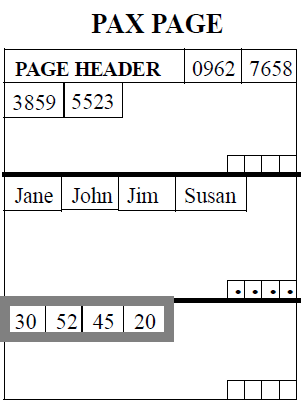
\includegraphics[width=3cm]{pax.png}};
\end{tikzpicture}

\begin{tikzpicture}[remember picture,overlay]
    \node[xshift=-1.5cm,yshift=-6cm] at (current page.north east) {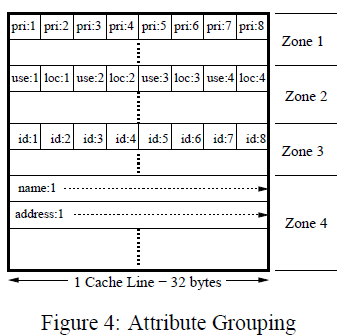
\includegraphics[width=3cm]{dmorphing.png}};
\end{tikzpicture}

\begin{tikzpicture}[remember picture,overlay]
    \node[xshift=-6cm,yshift=-7cm] at (current page.north east) {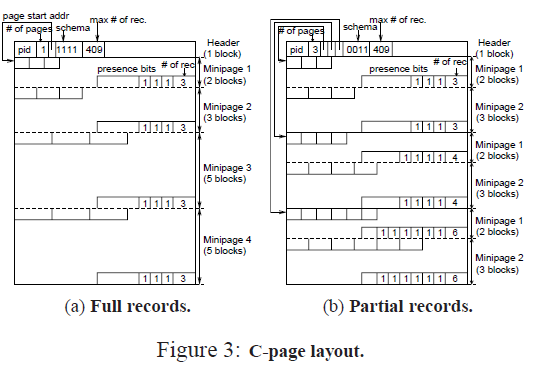
\includegraphics[width=4cm]{clotho.png}};
\end{tikzpicture}

\begin{tikzpicture}[remember picture,overlay]
    \node[xshift=-10cm,yshift=-7cm] at (current page.north east) {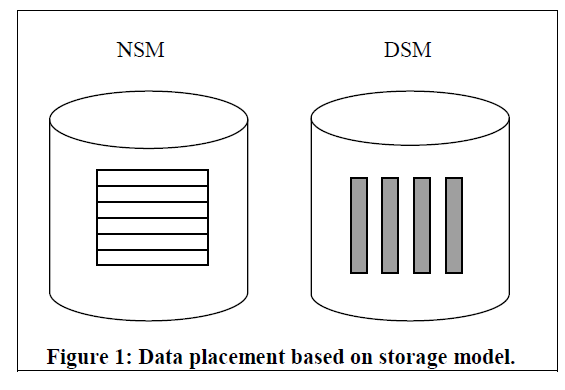
\includegraphics[width=4cm]{fractured-1.png}};
\end{tikzpicture}

\end{frame}

\begin{frame}
\frametitle{Обработка запроса во fractured mirrors (идея)}

Там была не только переработка buffer pool, а настоящая поколоночная обработка!
\\~\\
Q1: select ... from lineitem where l\_shipdate => date '1998-12-01' - interval '[DELTA]' day groupby ... orderby ...\\~\\

\begin{figure}[htb]
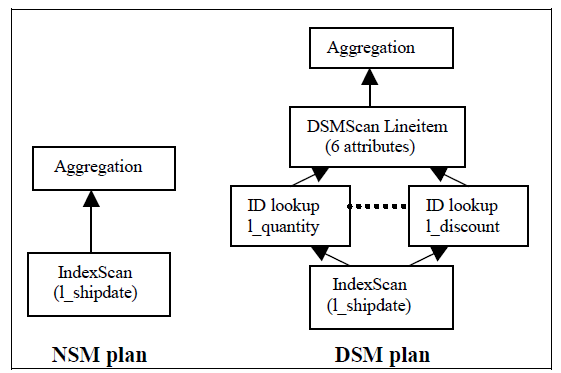
\includegraphics[width=\textwidth,height=0.50\textheight,keepaspectratio]{fractured-2.png}
 \end{figure}    

\end{frame}

\begin{frame}
\frametitle{Два подхода к колоночным СУБД\footnote{Есть немного на русском здесь: \url{http://citforum.ru/database/articles/column\_vs\_row\_store/}}}

\begin{itemize}
  \setlength\itemsep{1em}
  \item C-Store~--- дисковая, опирается на порядки сортировки, сжатие, раннюю и позднюю материализацию, новые операторы соединения и оперирование над сжатыми данными;
  \item MonetDB~--- в оперативной памяти, упор на эффективное использование железа: минимизация промахов в кешах кешей, использование хардварного параллелизма (SIMD). Специальная колоночная алгебра (BAT-алгебра), адаптивное индексирование, операторы для максимально эффективного использования железа. Тема 8 лекции.
\end{itemize}

\end{frame}

% todo: обмениваем диск на процессор

\begin{frame}
\frametitle{Общая архитектура дисковой колоночной системы}

\begin{itemize}
  \setlength\itemsep{1em}
  \item Каждая колонка хранится в отдельном файле;
  \begin{itemize}
    \item сжата, возможно своим алгоритмом;
    \item упорядочена согласно какомой-либо колонке (набору);
  \end{itemize}
  \item Наборов колонок может быть много (репликация);
  \item Операторы работают над одной колонкой или ``сборкой'' из нескольких;
  \item Между операторами ходят не только данные, но и ID записей;
  \item Когда ``менять'' ID на данные? Вопрос материализации.
\end{itemize}

Основная публикация: D. Abadi et al. Materialization Strategies in a Column-Oriented DBMS, 2007 IEEE 23rd International Conference on Data Engineering, Istanbul, 2007, pp. 466-475.

\end{frame}


\begin{frame}
\frametitle{Сжатие}

Один из столпов колоночной технологии. ``Обмениваем'' CPU на диск!

\begin{itemize}
  \setlength\itemsep{1em}
  \item До колоночной эры сжатие было, но другое: 
  \begin{itemize}
    \item сжимали гетерогенные данные $\longrightarrow$ в 2-3 раза;
    \item более тяжеловесные методы сжатия;
    \item не было операторов работающих со сжатыми данными.
  \end{itemize}
  \item Легковесное, примененное к одной колонке:
  \begin{itemize}
    \item Экономит место на диске до 10 раз;
    \item Типы:
    \begin{itemize}
      \item RLE
      \item Bit-vector
      \item Frame of Reference (FoR)
      \item Differential
      \item ...
    \end{itemize}
    \item Сжатие/разжатие можно о-SIMD-ить: 
    \begin{itemize}
    	\item J. Wang et al., An Experimental Study of Bitmap Compression vs. Inverted List Compression, SIGMOD 2017
    	\item P. Damme et al., Insights into the Comparative Evaluation of Lightweight Data Compression Algorithms, EDBT 2017
    \end{itemize}
  \end{itemize}
\end{itemize}

\end{frame}

\begin{frame}
\frametitle{Сжатие: RLE}

\begin{figure}[htb]
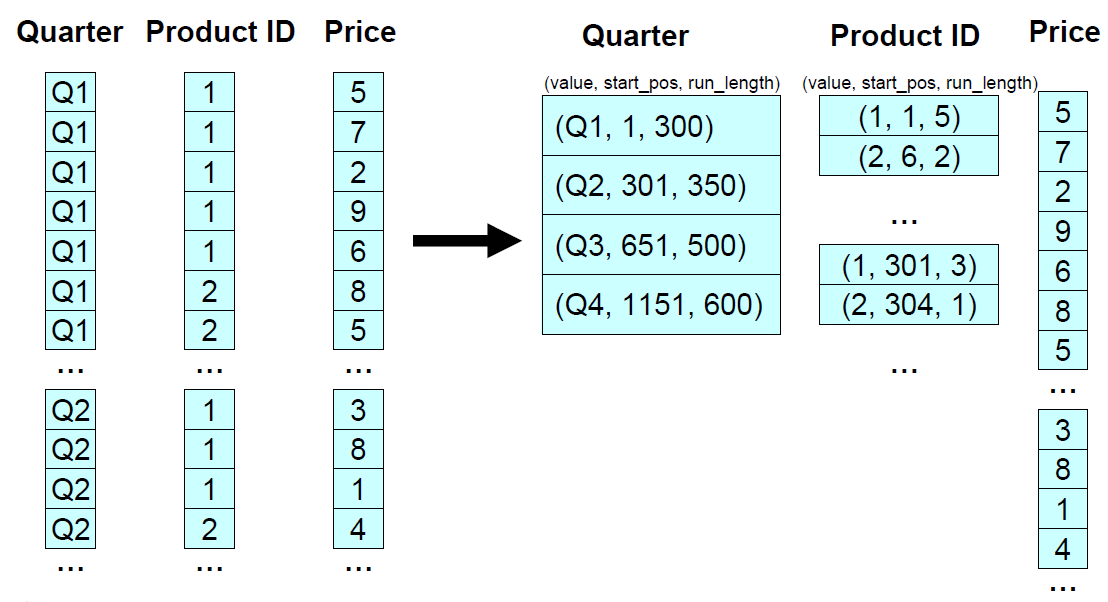
\includegraphics[width=\textwidth,height=0.75\textheight,keepaspectratio]{compression1.png} 
\footnote{\tiny{Изображение взято из \cite{Harizopoulos2009}}}
 \end{figure}    

\end{frame}

\begin{frame}
\frametitle{Сжатие: bit-vector}

\begin{figure}[htb]
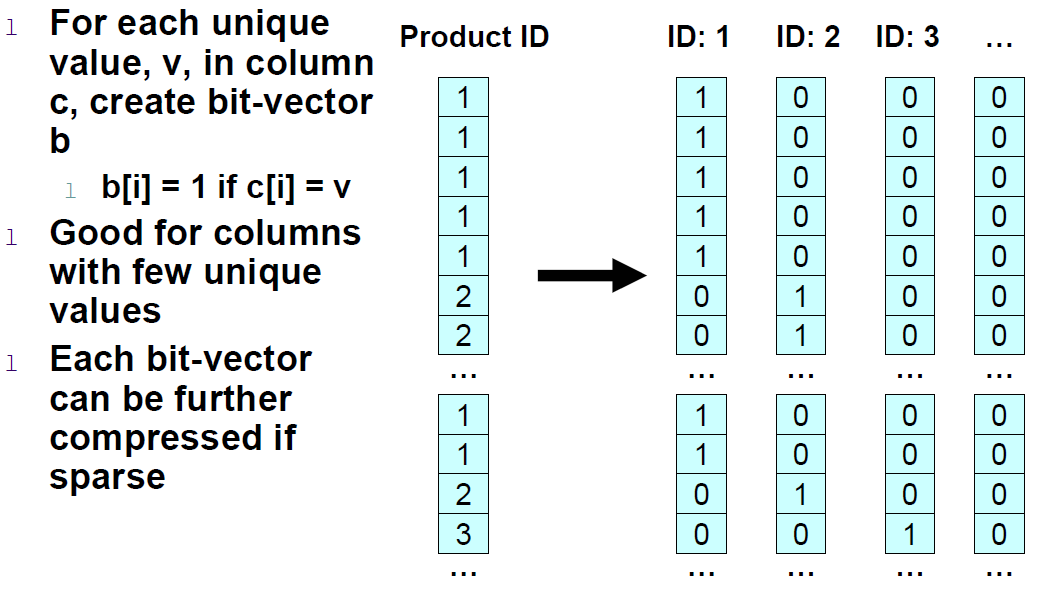
\includegraphics[width=\textwidth,height=0.75\textheight,keepaspectratio]{compression2.png} 
\footnote{\tiny{Изображение взято из \cite{Harizopoulos2009}}}
 \end{figure}    

\end{frame}

\begin{frame}
\frametitle{Сжатие: dictionary}

\begin{figure}[htb]
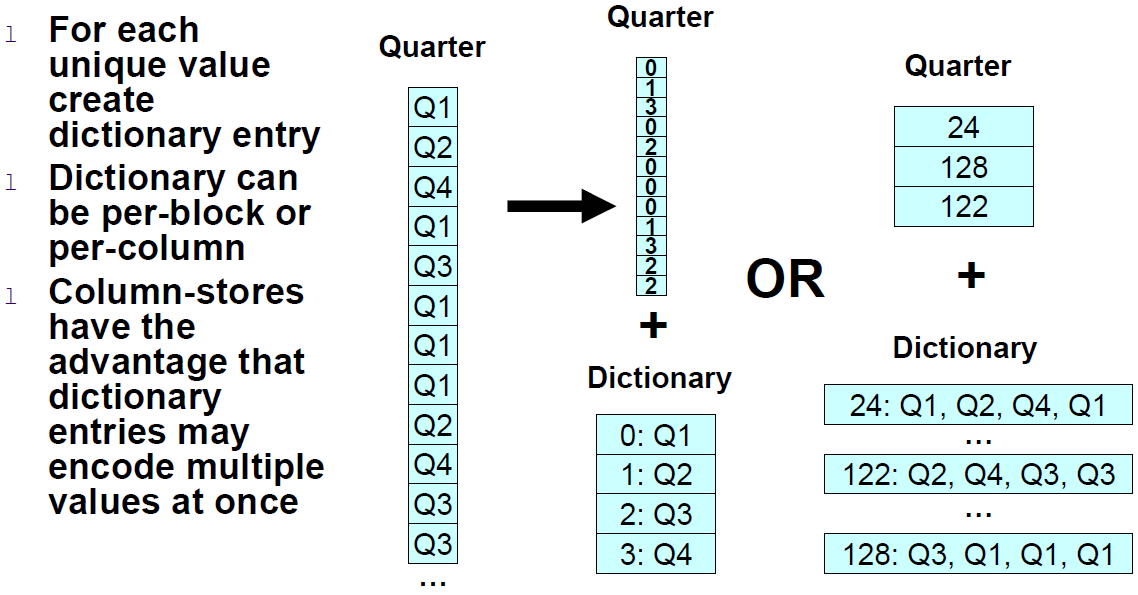
\includegraphics[width=\textwidth,height=0.75\textheight,keepaspectratio]{compression3.png} 
\footnote{\tiny{Изображение взято из \cite{Harizopoulos2009}}}
 \end{figure}    

\end{frame}

\begin{frame}
\frametitle{Сжатие: FoR}

\begin{figure}[htb]
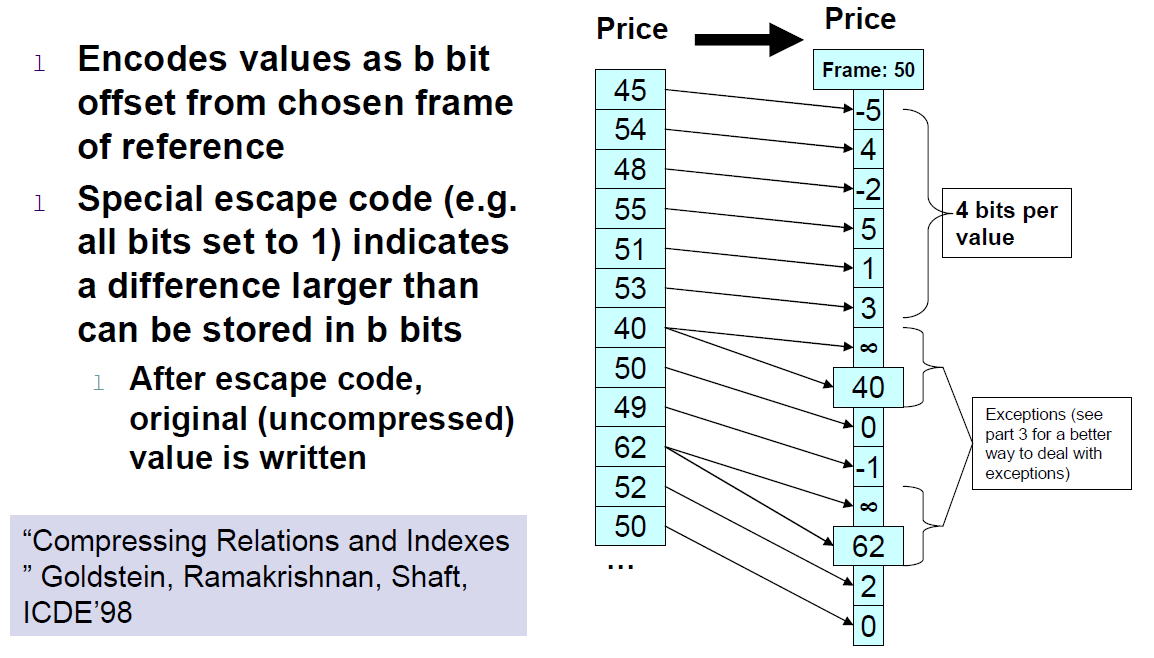
\includegraphics[width=\textwidth,height=0.75\textheight,keepaspectratio]{compression4.png} 
\footnote{\tiny{Изображение взято из \cite{Harizopoulos2009}}}
 \end{figure}    

\end{frame}

\begin{frame}
\frametitle{Сжатие: differential}

\begin{figure}[htb]
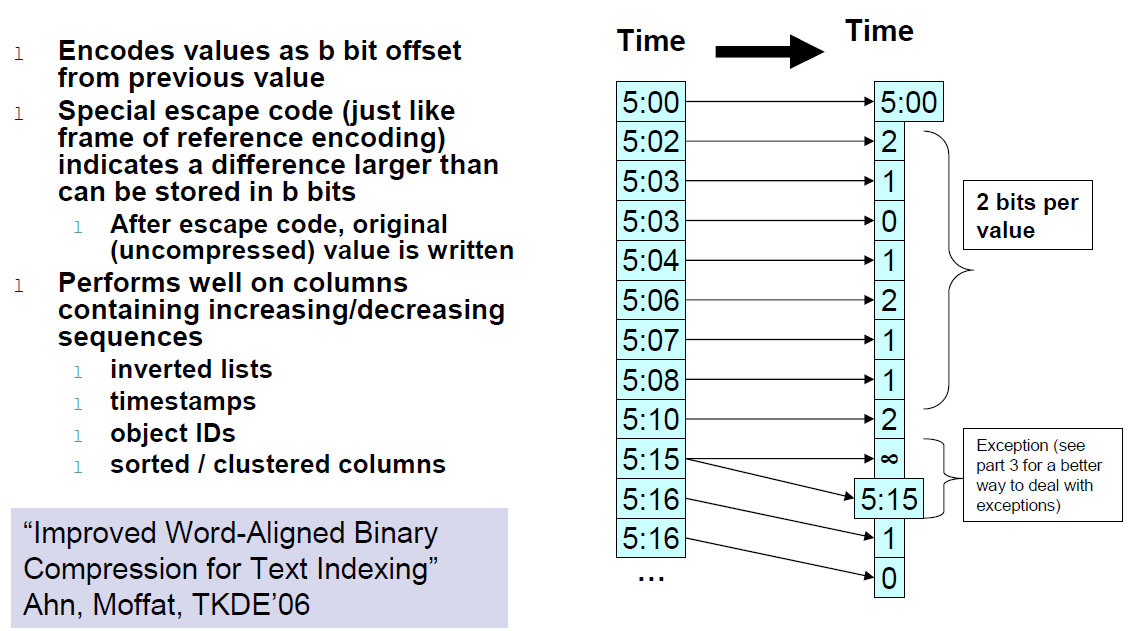
\includegraphics[width=\textwidth,height=0.75\textheight,keepaspectratio]{compression5.png} 
\footnote{\tiny{Изображение взято из \cite{Harizopoulos2009}}}
 \end{figure}    

\end{frame}

\begin{frame}
\frametitle{Сжатие: как выбирать алгоритм?}

\begin{figure}[htb]
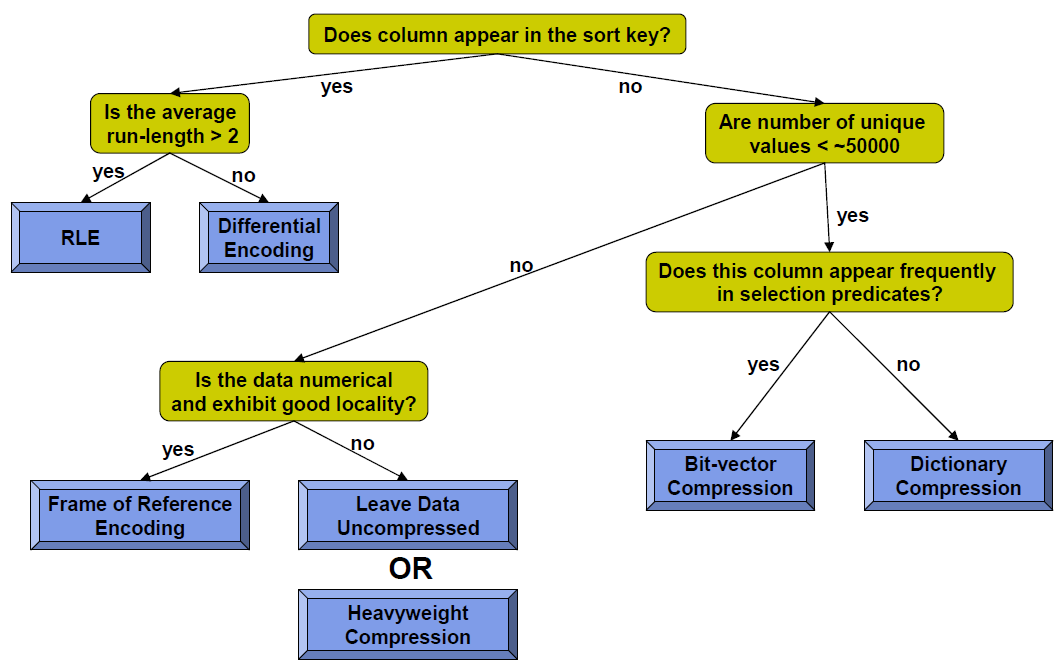
\includegraphics[width=\textwidth,height=0.75\textheight,keepaspectratio]{compression6.png} 
\footnote{\tiny{Изображение взято из \cite{Harizopoulos2009}}}
 \end{figure}    

\end{frame}

\begin{frame}
\frametitle{Почему легковесные схемы?}

\begin{figure}[htb]
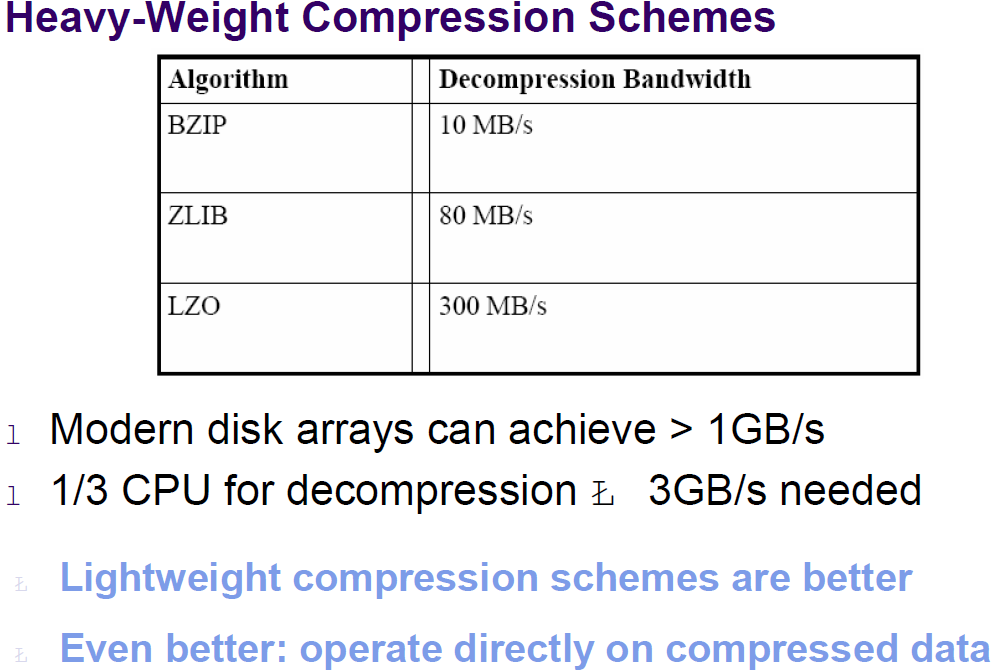
\includegraphics[width=\textwidth,height=0.75\textheight,keepaspectratio]{compression7.png} 
\footnote{\tiny{Изображение взято из \cite{Harizopoulos2009}}}
 \end{figure}    

\end{frame}

\begin{frame}
\frametitle{Операции над сжатыми данными I}

\begin{figure}[htb]
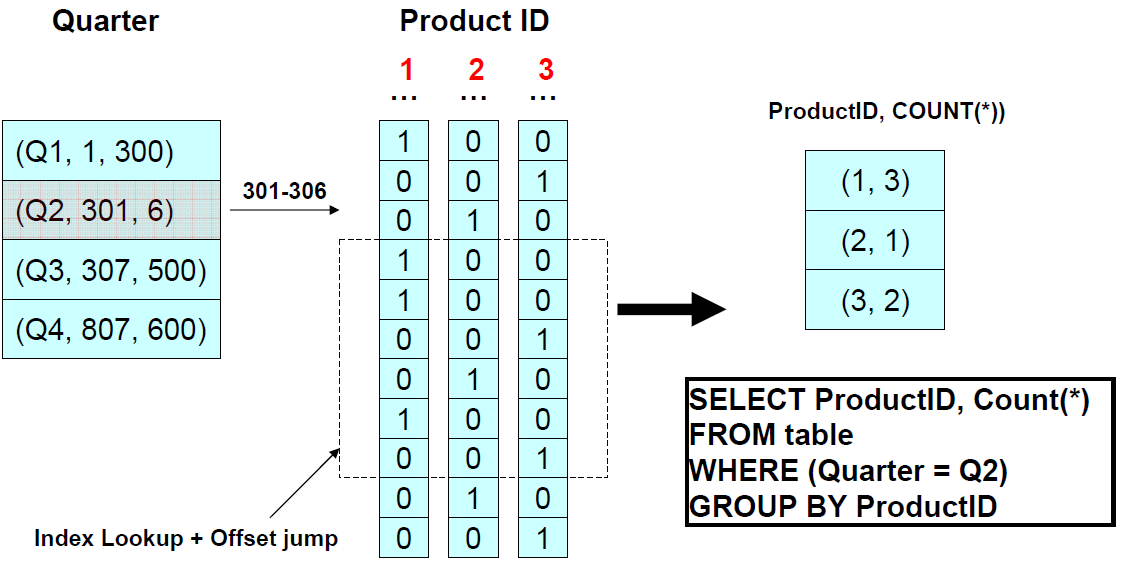
\includegraphics[width=\textwidth,height=0.75\textheight,keepaspectratio]{compression8.png} 
\footnote{\tiny{Изображение взято из \cite{Harizopoulos2009}}}
 \end{figure}    

\end{frame}

\begin{frame}
\frametitle{Операции над сжатыми данными II}

\begin{figure}[htb]
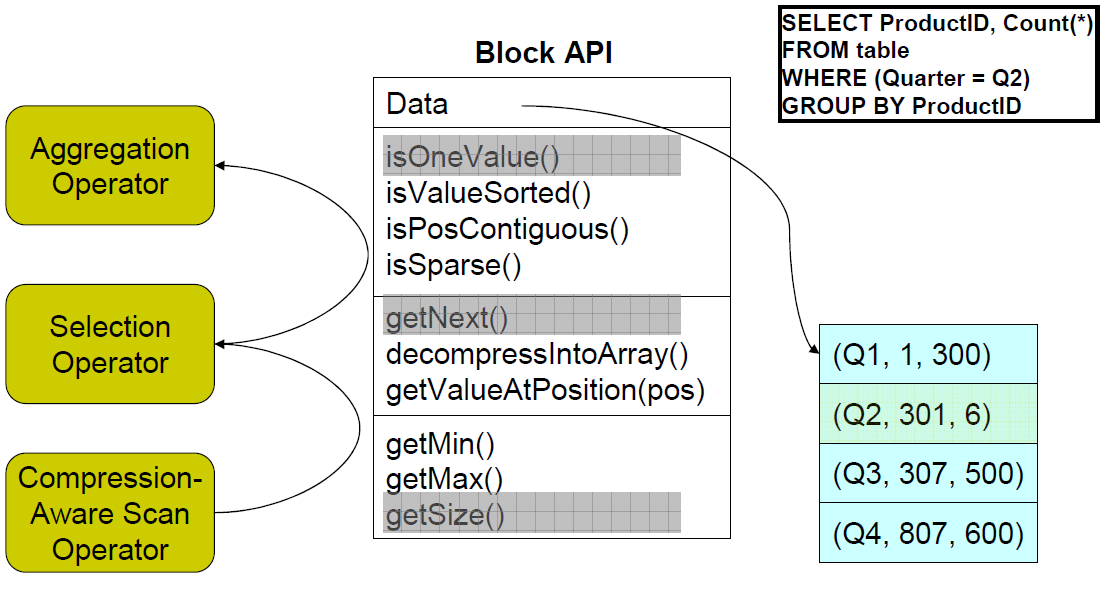
\includegraphics[width=\textwidth,height=0.75\textheight,keepaspectratio]{compression9.png} 
\footnote{\tiny{Изображение взято из \cite{Harizopoulos2009}}}
 \end{figure}    

\end{frame}


\begin{frame}
\frametitle{Исполнение запросов: материализация vs проекция}

Кажется что материализация это примерно проекция, однако...\\~\\

Проекция:
\begin{itemize}
  \setlength\itemsep{1em}
  \item В классических системах: выгодно как можно раньше;
  \item В колоночных системах: зависит!
  \begin{itemize}
    \item Материализация: считать нужные колонки и достать значения из нужных для конструирования ответа;
    \item Ранняя: в самом начале получить все нужные значения и выдавать наверх строки;
    \item Поздняя: максимально отложить этот процесс.
  \end{itemize}
\end{itemize}

Ранняя: проста в понимании и реализации, дешева с вычислительной точки зрения и точно \alert{всегда} дает выигрыш за счет эффективной работы с диском (сжатие, SIMD, игнорирование ненужных колонок). Поздняя: гораздо сложнее делать, но может быть \alert{дополнительный} выигрыш.

\end{frame}

\begin{frame}
\frametitle{Исполнение запросов: EM пример}

\begin{figure}[htb]
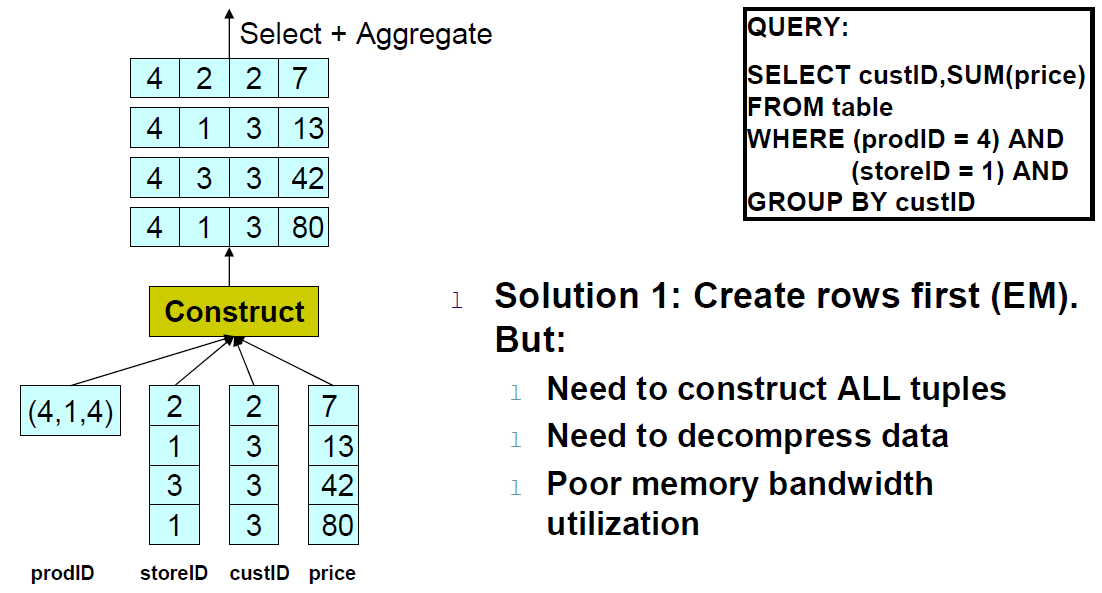
\includegraphics[width=\textwidth,height=0.75\textheight,keepaspectratio]{em.png} 
\footnote{\tiny{Изображение взято из \cite{Harizopoulos2009}}}
 \end{figure}    

\end{frame}

\begin{frame}
\frametitle{Исполнение запросов: LM пример I}

\begin{figure}[htb]
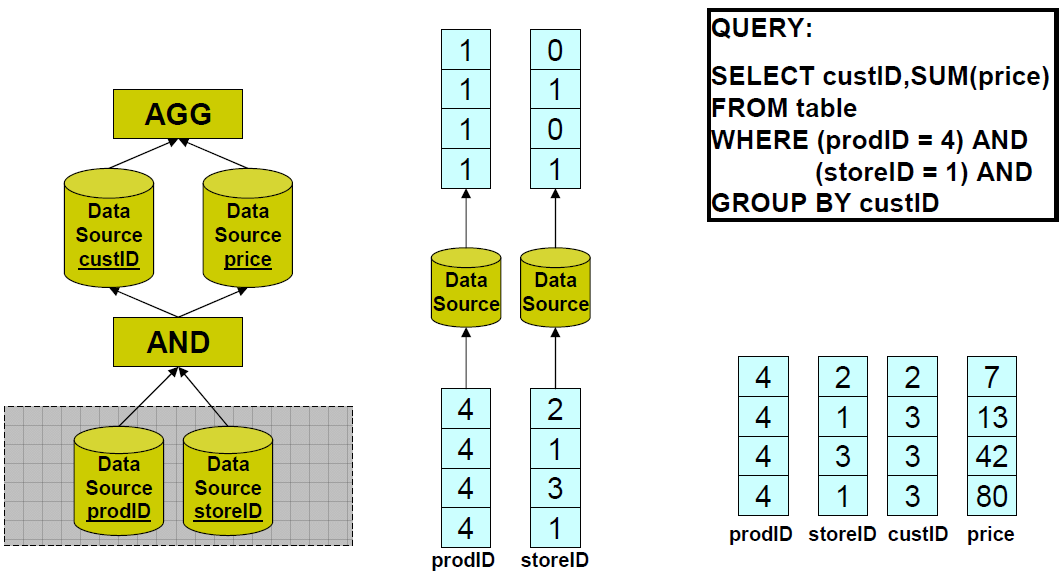
\includegraphics[width=\textwidth,height=0.75\textheight,keepaspectratio]{lm1.png} 
\footnote{\tiny{Изображение взято из \cite{Harizopoulos2009}}}
 \end{figure}    

\end{frame}

\begin{frame}
\frametitle{Исполнение запросов: LM пример II}

\begin{figure}[htb]
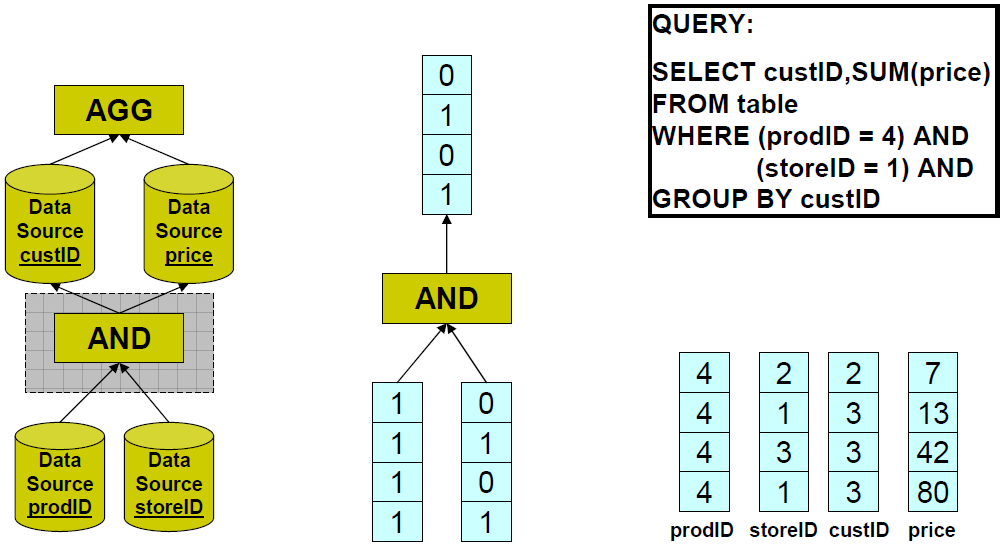
\includegraphics[width=\textwidth,height=0.75\textheight,keepaspectratio]{lm2.png} 
\footnote{\tiny{Изображение взято из \cite{Harizopoulos2009}}}
 \end{figure}    

\end{frame}

\begin{frame}
\frametitle{Исполнение запросов: LM пример III}

\begin{figure}[htb]
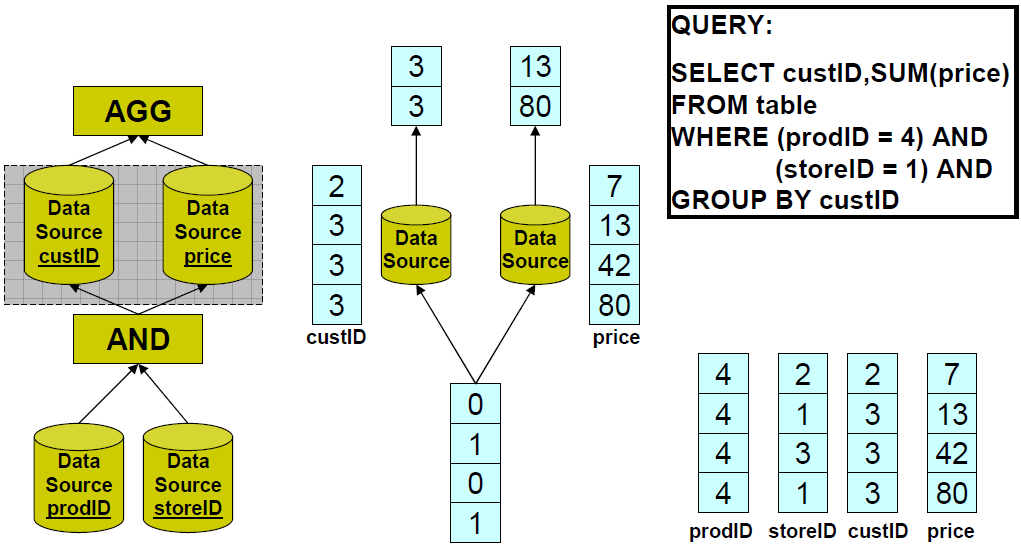
\includegraphics[width=\textwidth,height=0.75\textheight,keepaspectratio]{lm3.png} 
\footnote{\tiny{Изображение взято из \cite{Harizopoulos2009}}}
 \end{figure}    

\end{frame}

\begin{frame}
\frametitle{Исполнение запросов: LM пример IV}

\begin{figure}[htb]
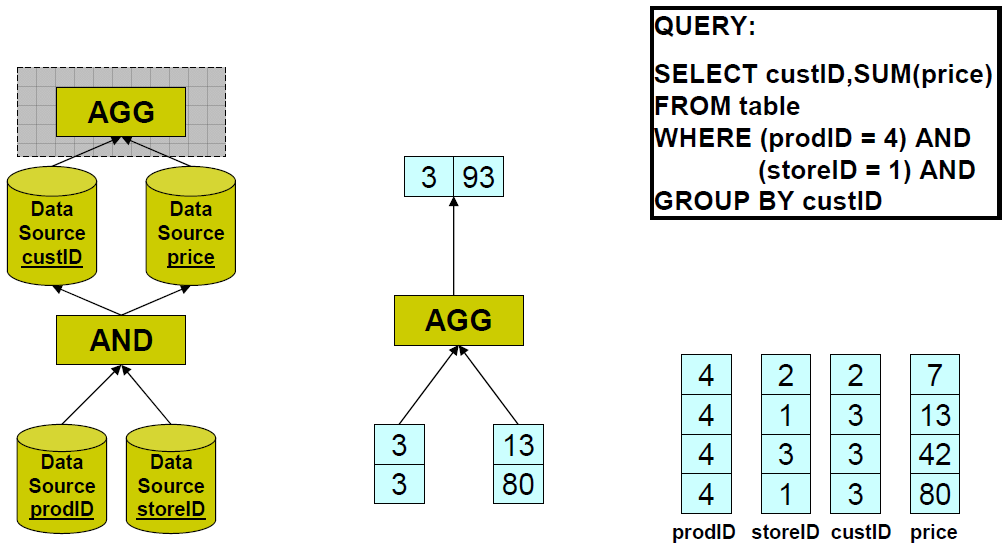
\includegraphics[width=\textwidth,height=0.75\textheight,keepaspectratio]{lm4.png} 
\footnote{\tiny{Изображение взято из \cite{Harizopoulos2009}}}
 \end{figure}    

\end{frame}


\begin{frame}
\frametitle{Что лучше, если нет соединений?}

\begin{figure}[htb]
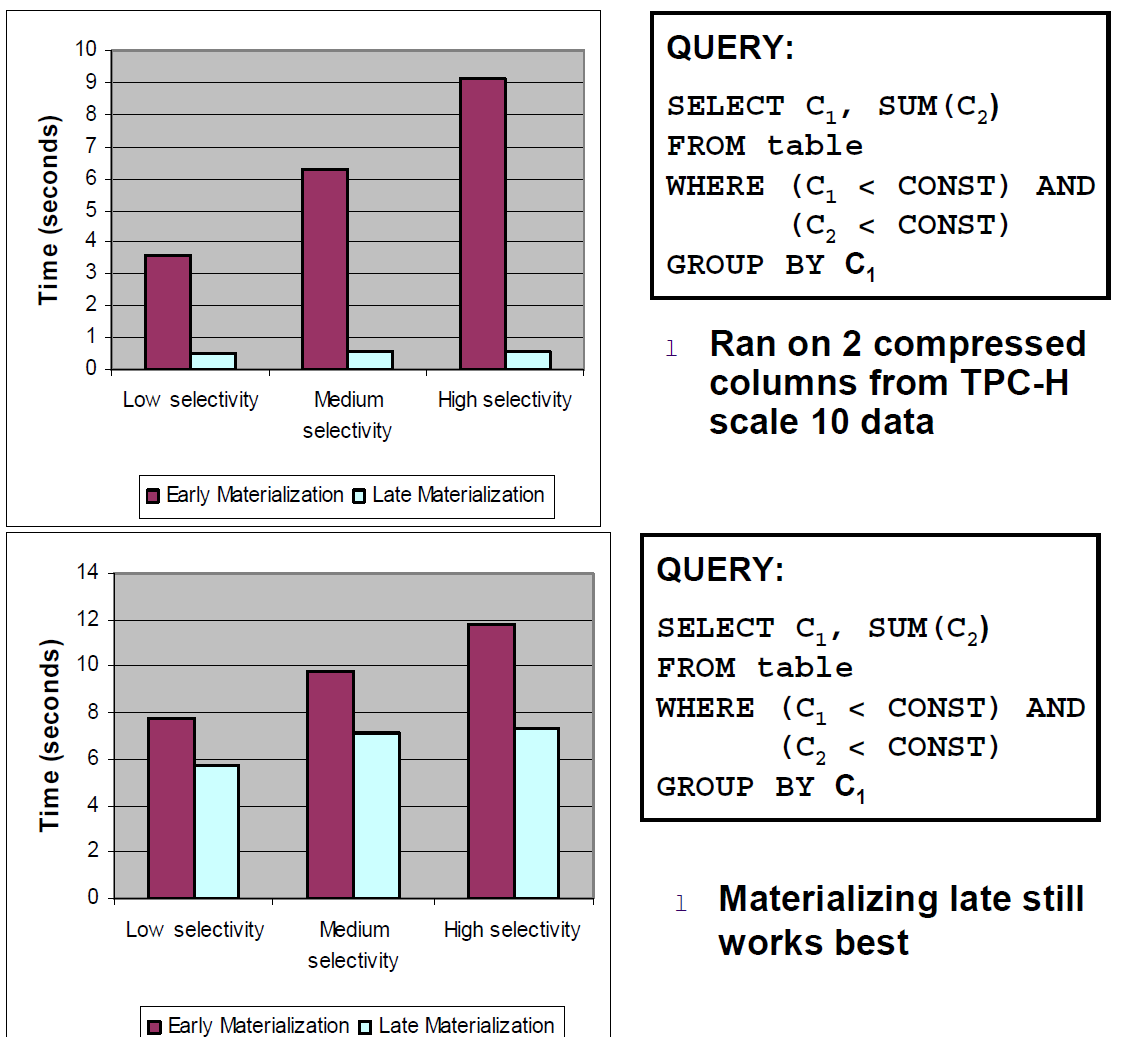
\includegraphics[width=\textwidth,height=0.75\textheight,keepaspectratio]{compare.png} 
\footnote{\tiny{Изображение взято из \cite{Harizopoulos2009}}}
 \end{figure}    

\end{frame}

\begin{frame}
\frametitle{Соединения}

\begin{figure}[htb]
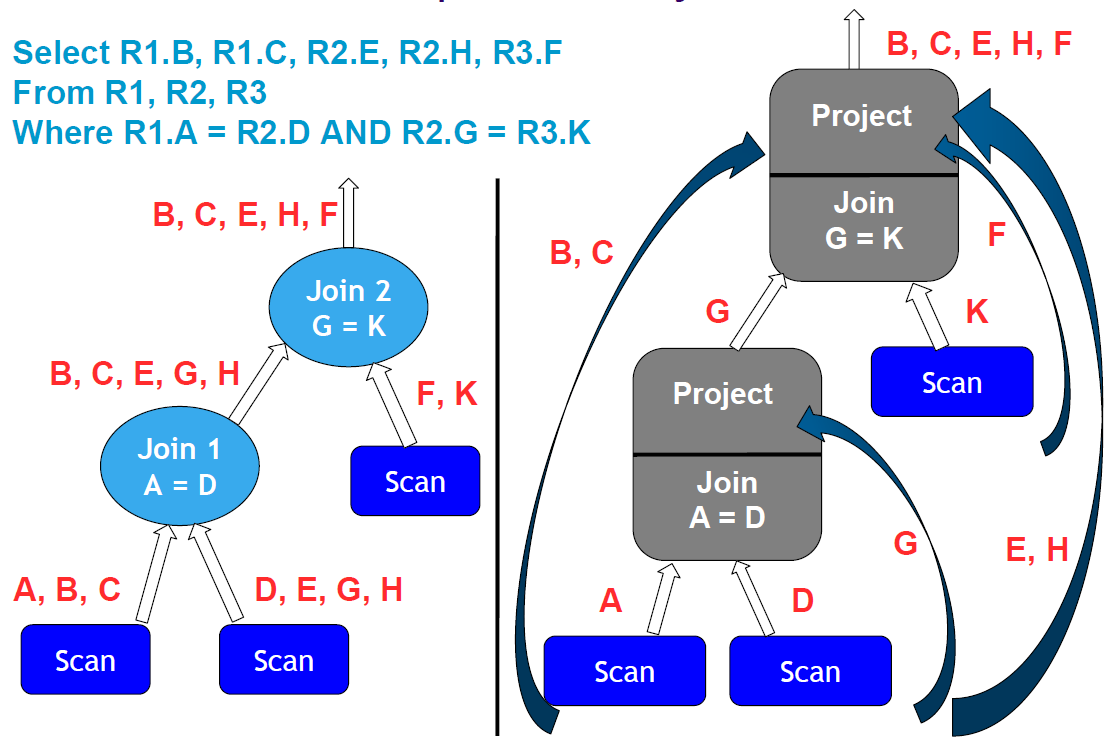
\includegraphics[width=\textwidth,height=0.75\textheight,keepaspectratio]{join1.png} 
\footnote{\tiny{Изображение взято из \cite{Harizopoulos2009}}}
 \end{figure}    

\end{frame}

\begin{frame}
\frametitle{Соединения и EM I}

\begin{figure}[htb]
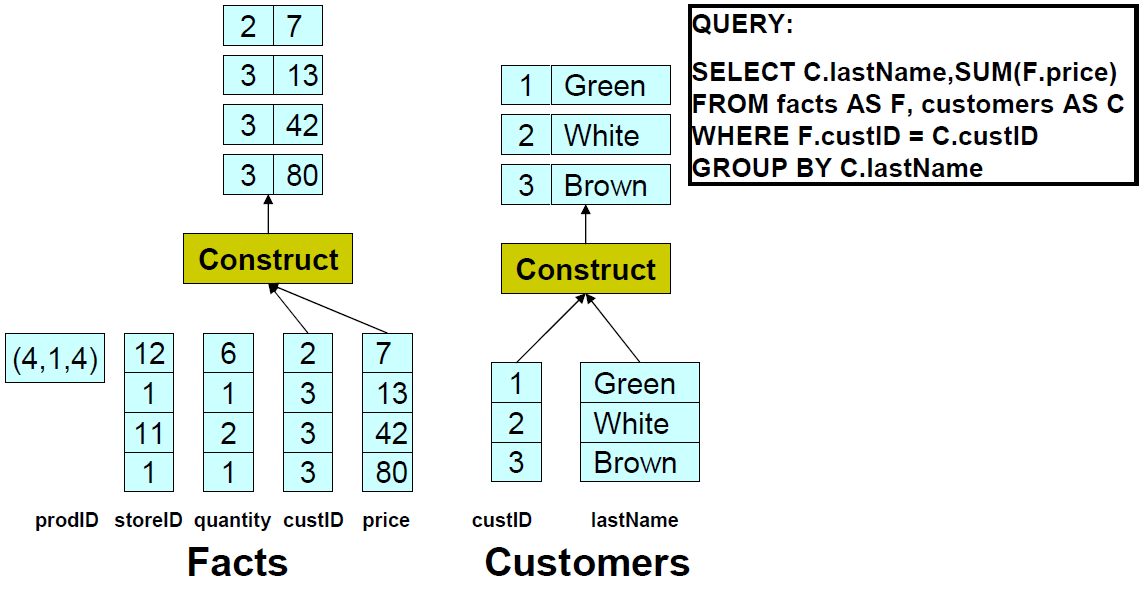
\includegraphics[width=\textwidth,height=0.75\textheight,keepaspectratio]{em-join1.png} 
\footnote{\tiny{Изображение взято из \cite{Harizopoulos2009}}}
 \end{figure}    

\end{frame}

\begin{frame}
\frametitle{Соединения и EM II}

\begin{figure}[htb]
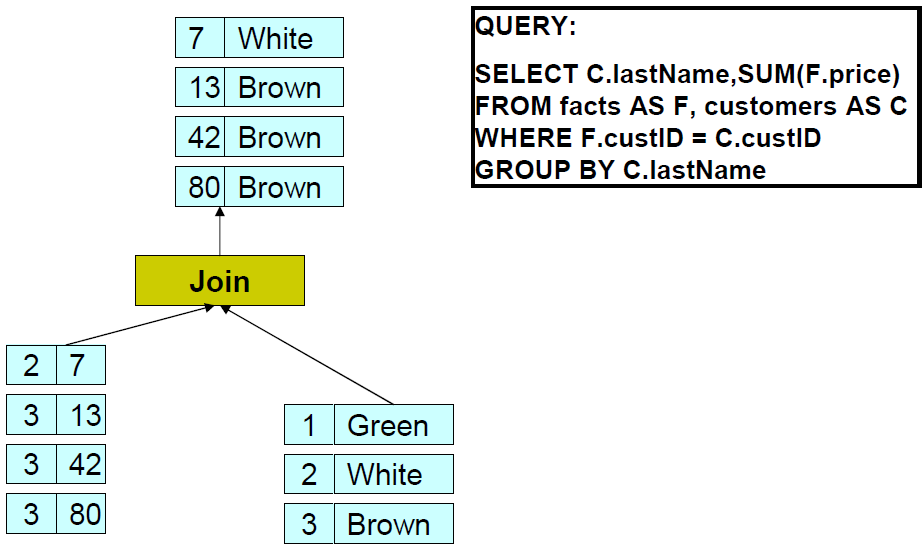
\includegraphics[width=\textwidth,height=0.75\textheight,keepaspectratio]{em-join2.png} 
\footnote{\tiny{Изображение взято из \cite{Harizopoulos2009}}}
 \end{figure}    

\end{frame}

\begin{frame}
\frametitle{Соединения и LM}

\begin{figure}[htb]
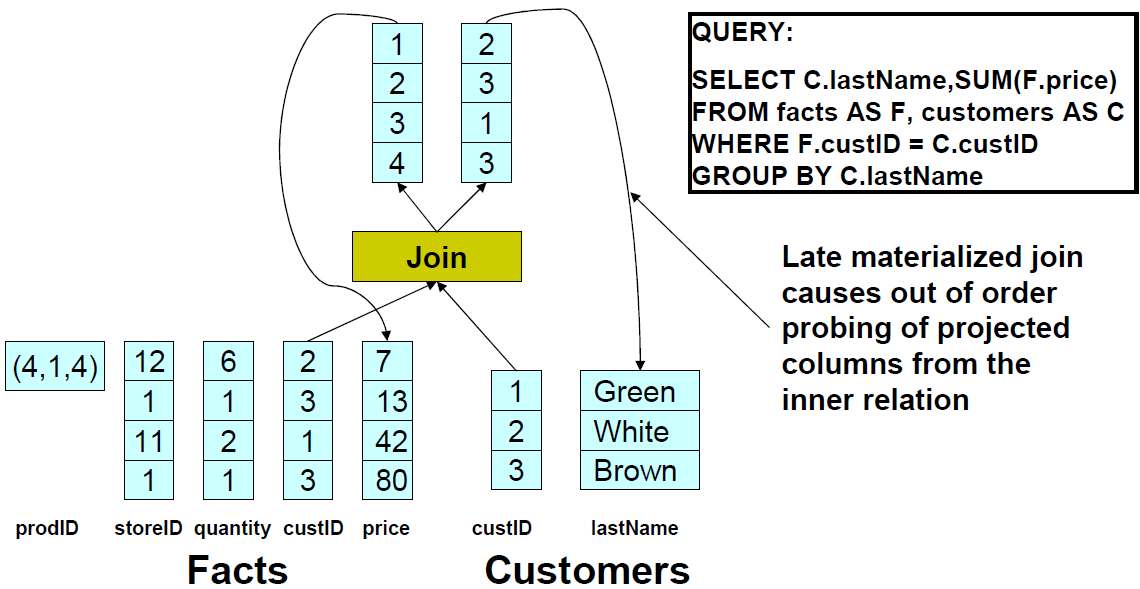
\includegraphics[width=\textwidth,height=0.75\textheight,keepaspectratio]{lm-join1.png} 
\footnote{\tiny{Изображение взято из \cite{Harizopoulos2009}}}
 \end{figure}    

\end{frame}

\begin{frame}
\frametitle{Промежуточный итог}

\begin{itemize}
  \setlength\itemsep{1em}
  \item Наивный LM в сочетании с соединением хуже в 2 раза (зависит от многих факторов, селективностей, объема памяти...) нежели EM;
  \item Ответ: новые алгоритмы соединения~--- на следующей лекции.
\end{itemize}

\end{frame}

\begin{frame}
\frametitle{Изображения}

Большинство изображений взяты из оригиналов статей или прямо из слайдов \cite{Harizopoulos2009}.

\end{frame}


\begin{frame}[allowframebreaks]
\frametitle{Ссылки}
\footnotesize{
\begin{thebibliography}{99}

\bibitem[Abadi et al., 2012] {Abadi2013} Daniel Abadi, Peter Boncz, Stavros Harizopoulos. The Design and Implementation of Modern Column-Oriented Database Systems. Foundations and Trends(R) in Databases Vol. 5, No. 3 (2012) 197--280

\bibitem[Harizopoulos et al., 2009] {Harizopoulos2009} Stavros Harizopoulos, Daniel Abadi, Peter Boncz. Column-Oriented Database Systems. VLDB 2009 Tutorial (slides).

\bibitem[Чернышев, 2013] {Chernishev2013}	Г. А. Чернышев, <<Организация физического уровня колоночных СУБД>>, Тр. СПИИРАН, 30 (2013), 204--222

\bibitem[Кузнецов, 2010] {Kuznetsov2010}	 Кузнецов С.Д., << MapReduce: внутри, снаружи или сбоку от параллельных СУБД?>>, Труды Института системного программирования РАН, 19 (2010), 35--70

%\bibitem[Elnikety, 2009] {Elnikety2009} Distributed DBMS. Sameh Elnikety. Encyclopedia of Database Systems. Ling Liu and M. Tamer {\"O}zsu (eds), p. 896--899. Springer US, 2009. \url{http://dx.doi.org/10.1007/978-0-387-39940-9\_654}

%\bibitem[Kian-Lee Tan, 2009] {Kian-Lee2009} Distributed Database Systems. Kian-Lee Tan. Encyclopedia of Database Systems. Ling Liu and M. Tamer {\"O}zsu (eds), p. 894--896. Springer US, 2009. \url{http://dx.doi.org/10.1007/978-0-387-39940-9_701}

%\bibitem[{\"O}zsu and Valduriez, 2009] {Ozsu2011} {\"O}zsu M.T. and Valduriez P. Principles of Distributed Database Systems, 3rd ed. Prentice-Hall, 2011.

%\bibitem[Kossmann, 2000] {Kossmann2000} Donald Kossmann. 2000. The state of the art in distributed query processing. ACM Comput. Surv. 32, 4 (December 2000), 422--469. DOI=http://dx.doi.org/10.1145/371578.371598 


%\bibitem[Ioannidis, 2003] {Ioannidis2003}  Yannis Ioannidis. 2003. The history of histograms (abridged). In Proceedings of the 29th international conference on Very large data bases - Volume 29 (VLDB '03), Johann Christoph Freytag, Peter C. Lockemann, Serge Abiteboul, Michael J. Carey, Patricia G. Selinger, and Andreas Heuer (Eds.), Vol. 29. VLDB Endowment 19--30. 

%\bibitem[Ioannidis and Poosala, 1995] {Ioannidis1995} Y. Ioannidis and V. Poosala. Histogram Based Solutions to Diverse Database Estimation Problems, IEEE Data Engineering, Vol. 18, No. 3, pp. 10--18, September 1995.

%\bibitem[Poosala et al., 1996] {Poosala1996} Viswanath Poosala, Peter J. Haas, Yannis E. Ioannidis, and Eugene J. Shekita. 1996. Improved histograms for selectivity estimation of range predicates. In Proceedings of the 1996 ACM SIGMOD international conference on Management of data (SIGMOD '96), Jennifer Widom (Ed.). ACM, New York, NY, USA, 294--305. DOI=http://dx.doi.org/10.1145/233269.233342 


%\bibitem[Kooi, 1980] {Kooi1980} Robert Philip Kooi. The Optimization of Queries in Relational Databases. PhD Thesis, Case Western Reserve University (1980).

%\bibitem[Piatetsky-Shapiro and Connel, 1984] {Piatetsky-Shapiro1984} Gregory Piatetsky-Shapiro and Charles Connell. 1984. Accurate estimation of the number of tuples satisfying a condition. In Proceedings of the 1984 ACM SIGMOD international conference on Management of data (SIGMOD '84). ACM, New York, NY, USA, 256--276. DOI=http://dx.doi.org/10.1145/602259.602294 


%\bibitem[Garcia-Molina et al., 2004] {Ulman2004} Гектор Гарсиа-Молина, Джеффри Д. Ульман, Дженнифер Уидом. Системы баз данных. Полный курс.  ISBN 5-8459-0384-Х; 2004 г. 

%\bibitem[Hellerstein et al., 2007] {Hellerstein2007} Joseph M. Hellerstein, Michael Stonebraker, and James Hamilton. Architecture of a Database System. Found. Trends databases 1, 2 (February 2007), 141--259. 

%\bibitem[Neumann, 2009] {Neumann2009} Thomas Neumann. Query Optimization (in Relational Databases). Encyclopedia of Database Systems. Springer US, 2009. 2273--2278.\url{http://dx.doi.org/10.1007/978-0-387-39940-9_293}

%\bibitem[Selinger et al., 1979] {Selinger1979} Selinger P.G., Astrahan M.M., Chamberlin D.D., Lorie R.A., and Price T.G. Access path selection in a relational database management System. In Proc. ACM SIGMOD Int. Conf. on Management of Data, 1979, pp. 23--34.

%\bibitem[Haas et al., 1989] {Haas1989} Haas L.M., Freytag J.C., Lohman G.M., and Pirahesh H. Extensible query processing in starburst. In Proc. ACM SIGMOD Int. Conf. on Management of Data, 1989, pp. 377--388.

%\bibitem[Graefe, 1995] {Graefe1995} Graefe G. The cascades framework for query optimization. Q. Bull. IEEE TC on Data Engineering, 18(3):19--29, 1995.

%\bibitem[Graefe and McKenna, 1993] {Graefe1993} Graefe G. and McKenna W.J. The volcano optimizer generator: Extensibility and efficient search. In Proc. 9th Int. Conf. on Data Engineering, 1993, pp. 209--218.

%\bibitem[Chaudhuri, 1998] {Chaudhuri1998} Chaudhuri S. An overview of query optimization in relational systems. In Proc. 17th ACM SIGACT-SIGMOD-SIGART Symp. Principles of Database Systems, 1998, pp. 34--43.

%\bibitem[Ioannidis, 1996] {Ioannidis1996} Ioannidis Y. Query optimization. In Handbook of Computer Science, A.B. Tucker (ed.). CRC Press, 1996.

%\bibitem[Jarke and Koch, 1984] {Chaudhuri1984} Jarke M. and Koch J. Query optimization in database systems. ACM Comput. Surv., 16(2):111–152, 1984.

%\bibitem[Ioannidis, 1996] {Ioannidis1996} Yannis E. Ioannidis. 1996. Query optimization. ACM Comput. Surv. 28, 1 (March 1996), 121--123. DOI=http://dx.doi.org/10.1145/234313.234367 

%\bibitem[Graefe, 1996] {Graefe1996} Goetz Graefe. 1996. Iterators, schedulers, and distributed-memory parallelism. Softw. Pract. Exper. 26, 4 (April 1996), 427--452. DOI=http://dx.doi.org/10.1002/(SICI)1097-024X(199604)26:4<427::AID-SPE20>3.3.CO;2-8 

%\bibitem[Taniar et al., 2008] {Taniar2008} David Taniar, Clement H. C. Leung, Wenny Rahayu, and Sushant Goel. 2008. High Performance Parallel Database Processing and Grid Databases. Wiley Publishing. 

\bibitem[Ramakrishnan and Gehrke, 2000] {Ramakrishnan2000}  Raghu Ramakrishnan and Johannes Gehrke. 2000. Database Management Systems (2nd ed.). Osborne/McGraw-Hill, Berkeley, CA, USA. 

\end{thebibliography}
}
\end{frame}


\end{document} 